\section{libvirt}

\begin{frame}
	{libvirt}

	\textbf{libvirt} is an \texttt{open-source} management toolkit for managing 
	virtualization platforms. 

	The project home page is \url{https://libvirt.org/}
\end{frame}

\cprotect\note{

}

\begin{frame}
   {libvirt overview}

   \begin{figure}[H]
      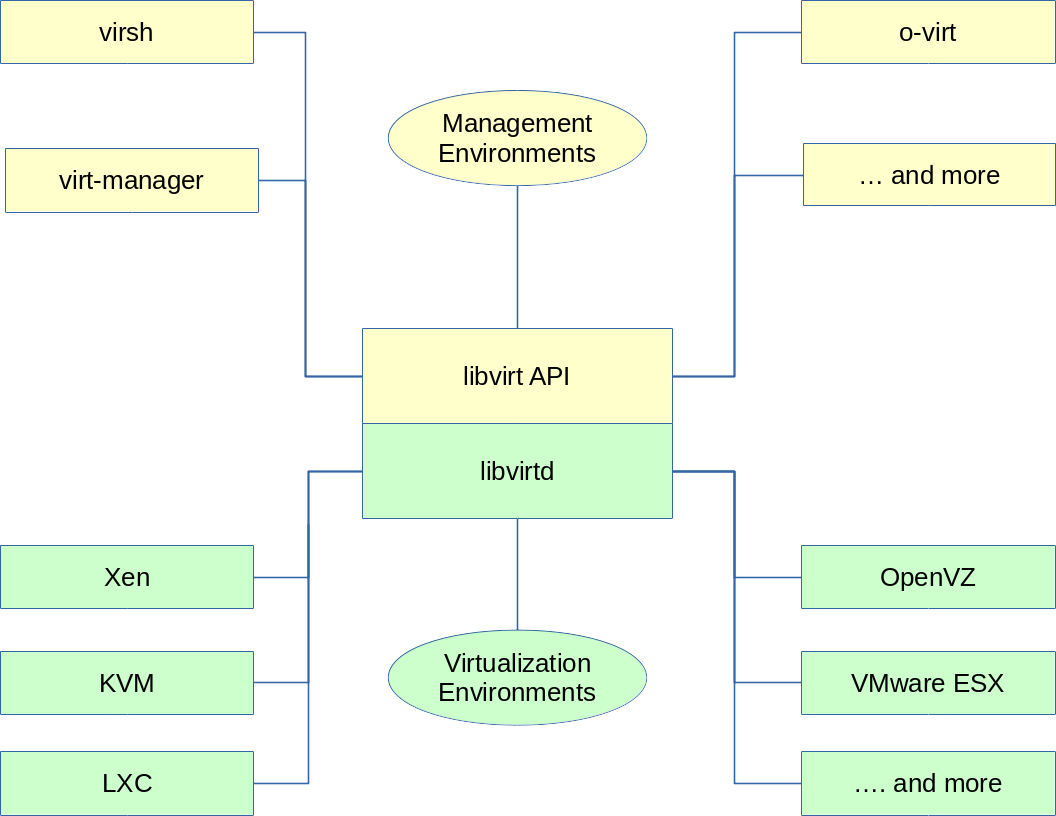
\includegraphics[height=3.2in]{IMAGES/libvirt-overview.png}
      \caption{Overview of libvirt}
   \end{figure}


\end{frame}

\cprotect\note{

	The package referred to as \textbf{libvirt} is comprised of two components:
	\begin{itemize}
	\item \textbf{libvirtd}, the server side daemon
		\begin{itemize}
			\item runs on host servers
			\item performs management tasks for virtual guests (start,stop,migrate,etc) 
		\end{itemize}
	\item \textbf{libvirt API} (client libraries and utilities) 
		\begin{itemize}
			\item connect to \textbf{libvirtd} via Unix socket or TCP/IP 
			\item request tasks be performed on the virtual guests
			\item request configuration and resource information
		\end{itemize}
	\end{itemize}

} 


\begin{frame}
   {libvirt-daemon overview}

   \begin{figure}[H]
      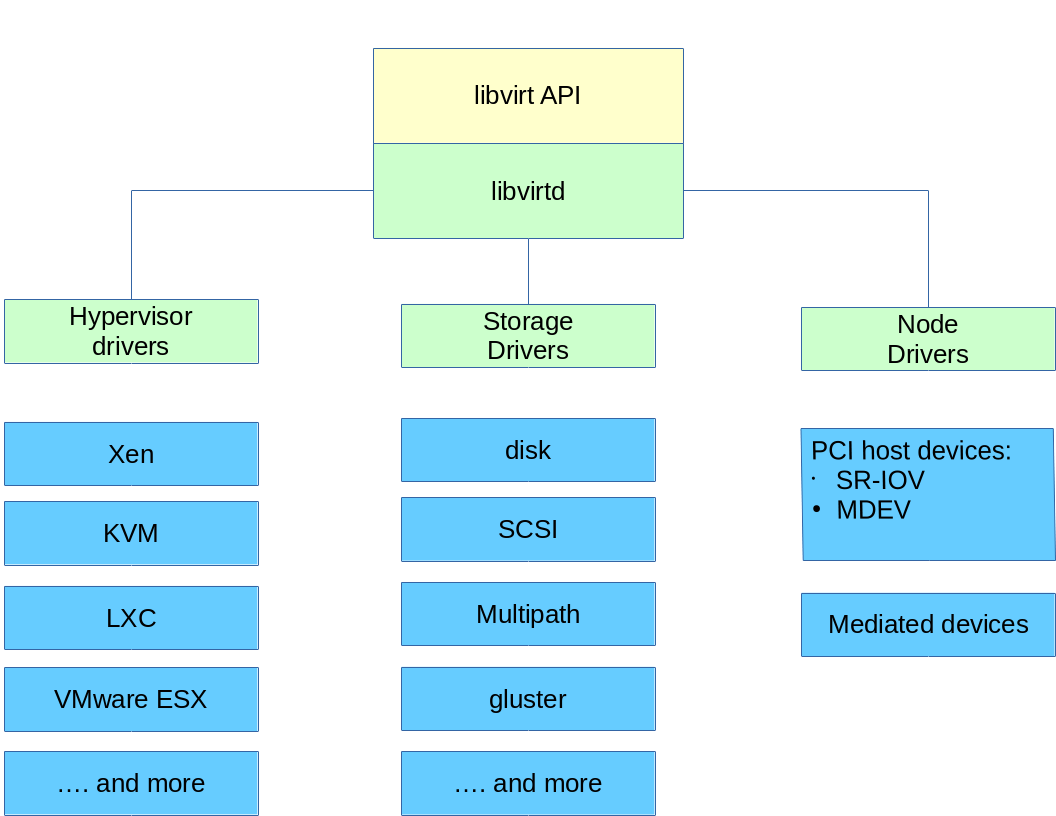
\includegraphics[height=3.2in]{IMAGES/kvm-libvirtd.png}
      \caption{Overview of libvirt-daemon}
   \end{figure}


\end{frame}


\cprotect\note{ 
	The \textbf{libvirtd} daemon is the component that is sensitive to various
	virtualization technologies. Generic input from the client library is translated
	to hypervisor specific commands, so a \textbf{vm start} command for a \textbf{xen}
	virtual machine is the same as a \textbf{vm start} command for a \textbf{kvm} virtual
	machine. Depending on the distribution there may be separate packages for the various 
	\textbf{libvirt-daemon} functions,  

   \begin{itemize}
      \item libvirt is a toolkit to manage virtualization technologies
      \begin{itemize}
         \item \textbf{KVM}/\textbf{QEMU}, \textbf{LXC}, \textbf{Xen}, \ldots and many more
      \end{itemize}
      \item libvirt provides an API interface usable by many different languages 
	      \begin{itemize}
		      \item \textbf{C, Python, Pearl},  \ldots and more
	      \end{itemize}
      \item libvirt provides management APIs for:
      \begin{itemize}
	 \item network filters, host devices, host interfaces, virtual networks,
         secrets, storage pools
	 \item for a complete list of the API support matrix see:
		\url{https://libvirt.org/hvsupport.html}
      \end{itemize}
   \end{itemize}


}


\begin{frame}
   {libvirtiAPI overview}

  {libvirtAPI overview}
   \begin{figure}[H]
      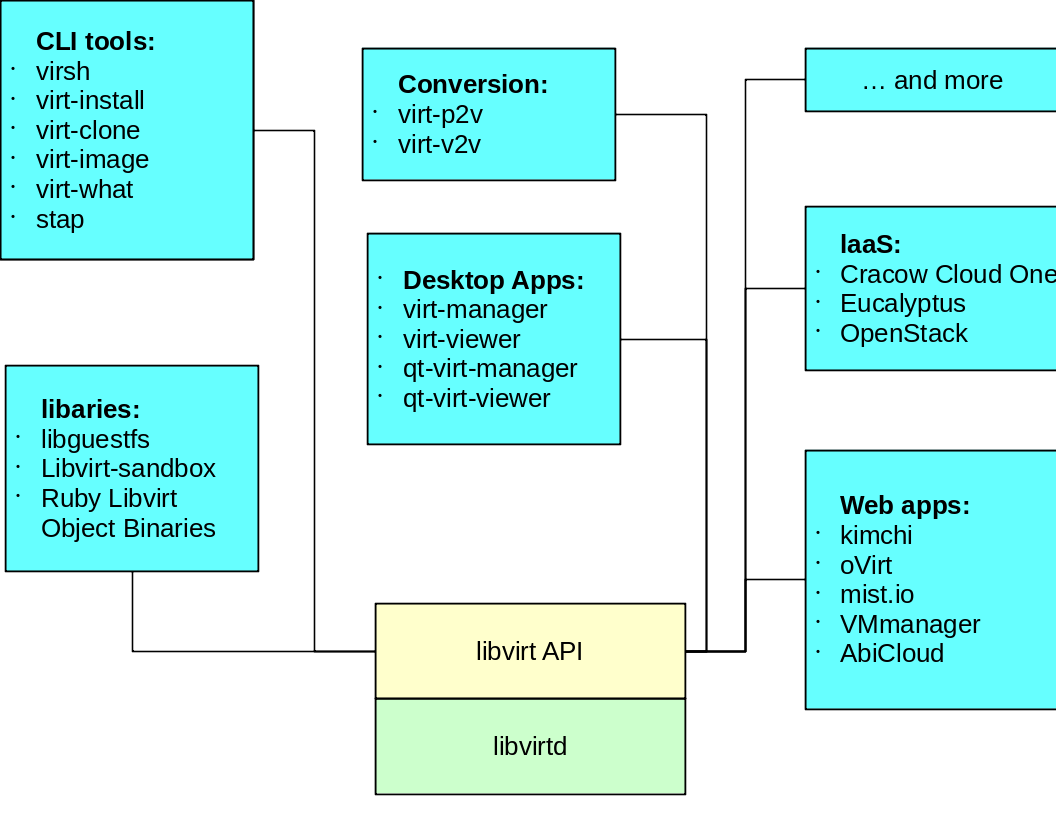
\includegraphics[height=3.2in]{IMAGES/kvm-libvirt-api.png}
      \caption{Overview of libvirtAPI}
   \end{figure}


\end{frame}

\cprotect\note{ 

 The \textbf{libvirt API} provides a common user interface to various
        virtualization environments. The connection to the virtualization environment is
        made by the \textbf{libvirtd} daemon running on the VM host. 
	Once the connection is established, applications
        can configure and control the virtual environments with 
	tools such as \textbf{virt-manager} or
        \textbf{virsh}.

   	The \textbf{libvirt} project utilities are available on
   	most distributions.  There are many application
   	programs that interface with \textbf{libvirt}, some of
   	the most common are \textbf{virt-manager},
   	\textbf{virt-viewer},\textbf{virt-install},\textbf{virsh}.

   The complete list of \textbf{libvirt} applications is
   available at \url{http://www.libvirt.org}.


	Tools that use the \textbf{libvirtAPI} are in these genral categories:
	\begin{itemize}
		\item Command Line Tools
		\item Conversion Tools
		\item Desktop Multi-function Applications
		\item Web Applications
		\item Infrastructure as a service (IaaS)
	\end{itemize}

} 

